\chapter{Systems Evaluation}
\label{chptr:evaluation}



%In this chapter, an example scenario and its requirements are presented.
%Therefore, a risk analysis is made, a data model is presented and a high level analysis towards reliability and safety is conducted.
%Finally, different possible system patterns are presented and compared based on their reliability, practicability and comparability with the \gls*{DCPS}.

\section{Scenario Description}
\todo{Find better title}

As already explained before, the system will be located within the context of ~\gls*{ETCS}.
Information in \gls*{ETCS} can be quite diverse, all in terms of type, size, durability, actualization frequency, priority.
For example, the trains position is a small, periodically and frequently updated type of information, while a \gls*{MA} is valid for a longer time and may be updated unfrequently.
There is also a difference in whether the information is kept as a state of the system, or if it is provided as system input, that needs to be consumed and processed.

In this section, an overview about different information types and possibilities for their representation in \gls*{DDS} topics is specified.

\begin{table}[h!]
	\begin{center}
		\caption{\Gls*{QOS} policies for events in a \gls*{DDS} system.}
		\label{tab:eventQOS}
		\begin{tabularx}{\textwidth}{|X|X|X|}
			\hline
			\textbf{QoS policy} & \textbf{Setting} & \textbf{Description}\\
			\hline \hline
			Deadline & Depends on actual implementation & For periodically updating events, a deadline can be specified to detect when events are missing in a period. \\
			\hline
			DestinationOrder & SourceTimestamp & The event samples should be ordered based on the time they got produced. \\
			\hline
			Durability & Depends on actual implementation & It might be appropriate to let late joining DataReaders process the events. \\
			\hline
			History & KeepAll & All events shall eventually be send and processed. Therefore, the event samples should be stored on both the sender and the receiver side.  \\
			\hline
			Lifespan & Depends on actual implementation & A event may be only valid for a specific period of time. This timespan can be specified by assigning a ifespan to a DataWriter. \\
			\hline
			Reliability & Reliable & The middleware will attempt to deliver all event data samples and actively checks if the receivers got them. In case the samples got lost, they are re-transmitted. \\
			\hline
			ResourceLimits & Depends on actual implementation & It might be appropriate to specify an upper bound for resouces to be allocated. Especially with History set to KeepAll. \\
			\hline
			WriterDataLifecycle & autodispose\_unregistered\-\_instances = False & Unregistered data instances should not be disposed because the events are required to be eventually processed. \\
			\hline
		\end{tabularx}
	\end{center}
\end{table}

A train's speed, as input data, is an example of data that needs to be eventually read and processed.
This kind of data can be summarized in the concept of events.
\autoref{tab:eventQOS} provides an overview about \gls*{QOS}-policy settings for event topics.
While some settings are common for event topics, some others need to be evaluated with regards to an actual system implementation and consequential requirements.

\begin{table}[h!]
	\begin{center}
		\caption{\Gls*{QOS} policies for volatile and enduring states in a \gls*{DDS} system.}
		\label{tab:stateQOS}
		\begin{tabularx}{\textwidth}{|X|X|X|X|}
			\hline
			\textbf{QoS policy} & \textbf{Setting for volatile state} & \textbf{Setting for enduring state} & \textbf{Description}\\
			\hline \hline
			Deadline & Depends on actual implementation & Not required & For volatile state, the deadline should match the period in which the data updates. Because enduring state is changing irregularly, it is not possible to define deadlines. \\
			\hline
			DestinationOrder & SourceTimestamp & SourceTimestamp & Using the source timestamp as ordering guarantees that always the most recent data is stored. However, this also requires a common clock for the distributed system. \\
			\hline
			Durability & Volatile & Transient or Persistent & Since volatile state is updated frequently, it is no problem when late joining subscribers miss previouly published data. The opposite is the case for slowly changing state, however. \\
			\hline
			History & KeepLast(n) & KeepLast(n) & Most of the time, only the last state matters, which is why n is typically set to one. \\
			\hline
			LatencyBudget & Depends on actual implementation & Not required & The maximum acceptable delay for sending the data should be choosen so that deadlines are not missed. \\
			\hline
			Reliability & BestEffort & Reliable & For rapidly and periodically changing state, it is ok if some data gets lost. For enduring state however, data has to be transferred reliably. \\
			\hline
			WriterDataLifecycle & Not required & autodispose\_unregistered\_instances = False & Event if data instances are unregistered, the actual data should not be disposed on enduring state topics. \\
			\hline
		\end{tabularx}
	\end{center}
\end{table}

While a train's speed could be periodically processed as an input information, it could also be kept as the system's state.
A state could contain perodically changing data, or irregular changing data, respectively.
A state that which data changes periodically is called a volatile state, while a state whose data changes slow and irregular is called enduring state.
Possible \gls*{QOS} settings for volatile and enduring states are presented in~\autoref{tab:stateQOS}.


%\subsection{High-Level Risk Analysis}

\section{System Design and Comparison}
The different redundancy techniques, as proposed, among others, by Johnson Barry, are applicable for different use-cases.
In this section, different redundancy techniques are selected, combined and evaluated based on following criteria:

\begin{itemize}
\item \textbf{Safety:} How likely is the system to reliable detect a failure and transition the system into a safe state.
\item \textbf{Implementability using \gls*{DDS}:} What ways are there to realize the redundancy with the \gls*{DDS} communication middleware.
\end{itemize}

In order to evaluate the redundant system's safety, it is mathematically evaluated using Marcov Chains, as described in~\autoref{sec:safetyEvaluation}.
For investigating the technique's implementability with \gls*{DDS}, the required functionalities, and \gls*{QOS} policies for setting up the architecture, are proposed and examined.
A datamodel will be carved out in \todo{Ref chapter 3}, when the proposed \gls*{DDS} architecture is implemented based on a real-life example.
One of the most commonly used techniques for building safe and fault-tolerant systems is \gls*{TMR}~\cite{FaultToleranceViaNMR}.
Therefore, \gls*{TMR} will be the starting point for system investigation in this thesis.

\subsection{Tripple Modular Redundancy}
\Gls*{TMR} was already briefly discussed in~\autoref{sec:redundancyPatterns} and depicted in~\autoref{fig:Classical2OO3}.
The reliability and safety characteristics of \gls*{TMR} has been studien in depth, for example by Arifeen \etal~\cite{ArifeenFaultTolerantTMR}.
Their findings show that the reliability of \gls*{TMR}-systems ($R_{TMR}(t)$), and thereby its intrinsic safety, is given by the sum of the probability of all three components functioning and two components functioning.

\begin{equation}
R_{TMR}(t) = 3e^{-2 \lambda t} - 2e^{-3 \lambda t}
\end{equation}

All four failure classes from~\autoref{sec:techniquesSafetyReliability} for at most one failing replica can be detected and masked by the system.
For example, if one replica produces a wrong result, the voter still receives two correct results and can mask the wrong result using a majority voting.
When more than one replica fails, only \textbf{F1}, \textbf{F2}, and \textbf{F3} can be detected.
If two or more replicas fail to produce on output within a certain time span, the voter can detect this as a deadline violation and can transfer the system in a safe state, e.g. by stopping the train.
However, when two or three replicas produce the same, wrong result, the voter erroneously accepts the wrong result as the majority.

If a replica is failing to deliver a correct result because of it not being internally consistent, \textbf{F4} can also be covered using component checking mechanisms.
In this way, the component checking results could be made public for the voter, so that corrupt replicas can be excluded from the voting process.
Therefore, when two replicas provide a wrong result and the voter knows that those two are not internally consistent, the correct result can still be derived from the last, functioning replica.


%------DDS-------
In order to map a redundant technique onto a \gls*{DDS} publish-/subscribe architecture, the core functionalities and \gls*{QOS} policies need to be defined.
The input stream can either be defined using \gls*{DDS} topics or directly wired.
If a \texttt{Input}-topic is used, it should be defined as an event to make sure that every replica receives and consumes the input.
Because input events cannot be planned, the deadline \gls*{QOS} is not applicable for input events.
Inputs typically require immediate processing and a maximal timespan $\Delta t$ from receiving the input to its final processing should be defined.
Therefore, its \texttt{Durability} can be set to volatile and the \texttt{Lifespan}-policy should be set to the difference between $\Delta t$ and the system's mean processing time for the considered input.
The input's \texttt{ResourceLimit} depends on the frequency the input is expected to be delivered.
\\

A replica's output should be implemented as an event topic, so that it can be ensured that the voter consumes and considers all replica outputs to process a final result.
For the \gls*{QOS}-settings applies the same as for the input topic's \gls*{QOS} settings.
The \texttt{Lifespan}-policy however should be set to the timespan that the voter expects all results to be ready and depends on the voter implementation.

As described earlier, voters can either be implemented in software, or in hardware.
When using \gls*{DDS} for the communication between the replicas and the voter, there always needs to be a software part involved in the voter that implements the \gls*{DCPS} standard.
\\

The individual component's internal consistency can either be monitored by the affected component itself, or by other components in the system.
In order to review whether a component has crashed, a periodical heartbeat message could be used.
A heartbeat message can be used to indicate the reachability of components or to synchronize them.
Information about internal consistency and reachability should be vetted in a fixed period and can be stored using a volatile \gls*{DDS} state.
The \texttt{Deadline} and \texttt{LatencyBudget} \gls*{QOS}-settings depend on the frequency that the monitoring takes place.

By using \abr{DDS} for exchanging system diagnosis data, such as heartbeat messages, it can also be ensured that the \abr{DDS} middleware is up and running on all monitored components.
In addition, the network latency can be reviewed.
The utilized topic should be implemented as an event to ensure that all monitoring messages are received and consumed by all replicas.
\\

However, the \abr{TMR} approach so far has the problem, that a failure of one component could make it a one-out-of-two system.
In one-out-of-two systems, majority voting is impossible.
In situations where the voter has to decide between two different results, it must choose the more restrictive one.
One way for the system to continue performing a majority voting even if an individual component fails, is by using active hardware redundancy.

\subsection{\Gls*{TMR} with spares}
\begin{figure}[!hb]
	\centering
	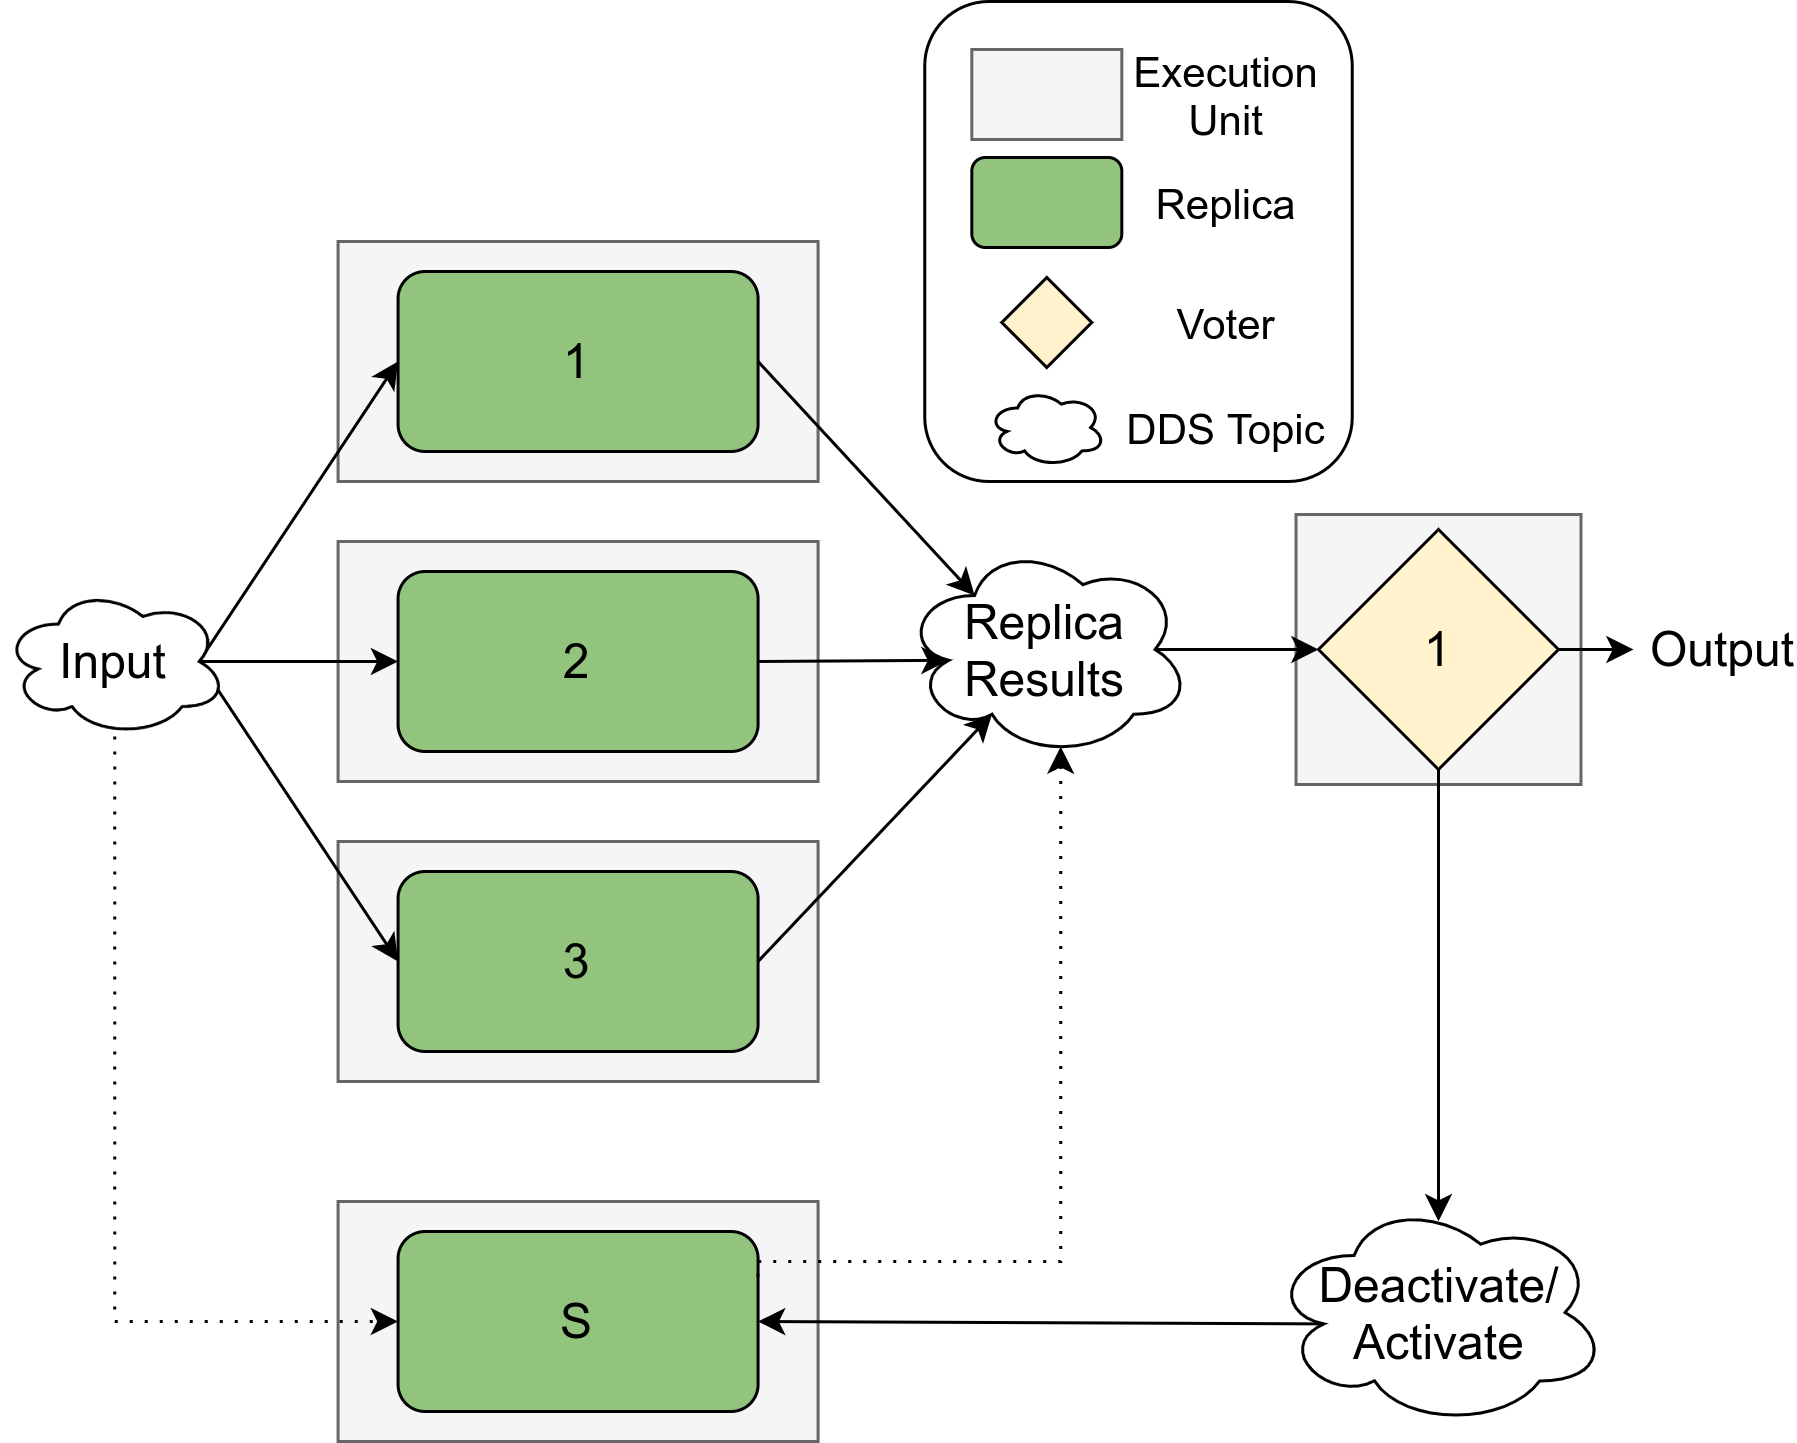
\includegraphics[width=0.75\linewidth]{images/TMRWithSparesDDS}
	\caption{A hot standby can be implemented using \abr{DDS} Topics for communication.}
	\label{fig:TMRWithSparesDDS}
\end{figure}

Standby redundancy is a way to keep a two-out-of-three system running even if an individual component fails.
It uses one or more spare components, which can be applied as a replacement for any component running in the system.
Implementing the entire system communication using \abr{DDS} can make the implementation of spares relatively easy, because a spare component can receive or publish data to a topic by simply connecting to it.
The concept is visalized in~\autoref{fig:TMRWithSparesDDS}, where a spare replica (S) replace a failed replica.
A failed replica can, for example, be identified by checking for its internal consistency or by using heartbeat messages.
As soon as the voter detects a failed replica, it can issue the spare replica (S) to subscribe to the input topic and publish data to the replica result topic.
A precondition for this to work is, that a replica's result can be unambiguously assigned to a replica, for example by using IDs or by using individual topics for each replica.
Because it allows one replica to fail without affecting the system's reliability, the reliability function changes for \abr{TMR} with spares.

\begin{equation}
R_{TMR\_S}(t) = 2 * {3 \choose 3} e^{-\lambda t} + {3 \choose 2} e^{-\lambda t}
 = 3e^{-2 \lambda t} - e^{-3 \lambda t}
\end{equation}

% Pipeline based
\begin{figure}[!hb]
	\centering
	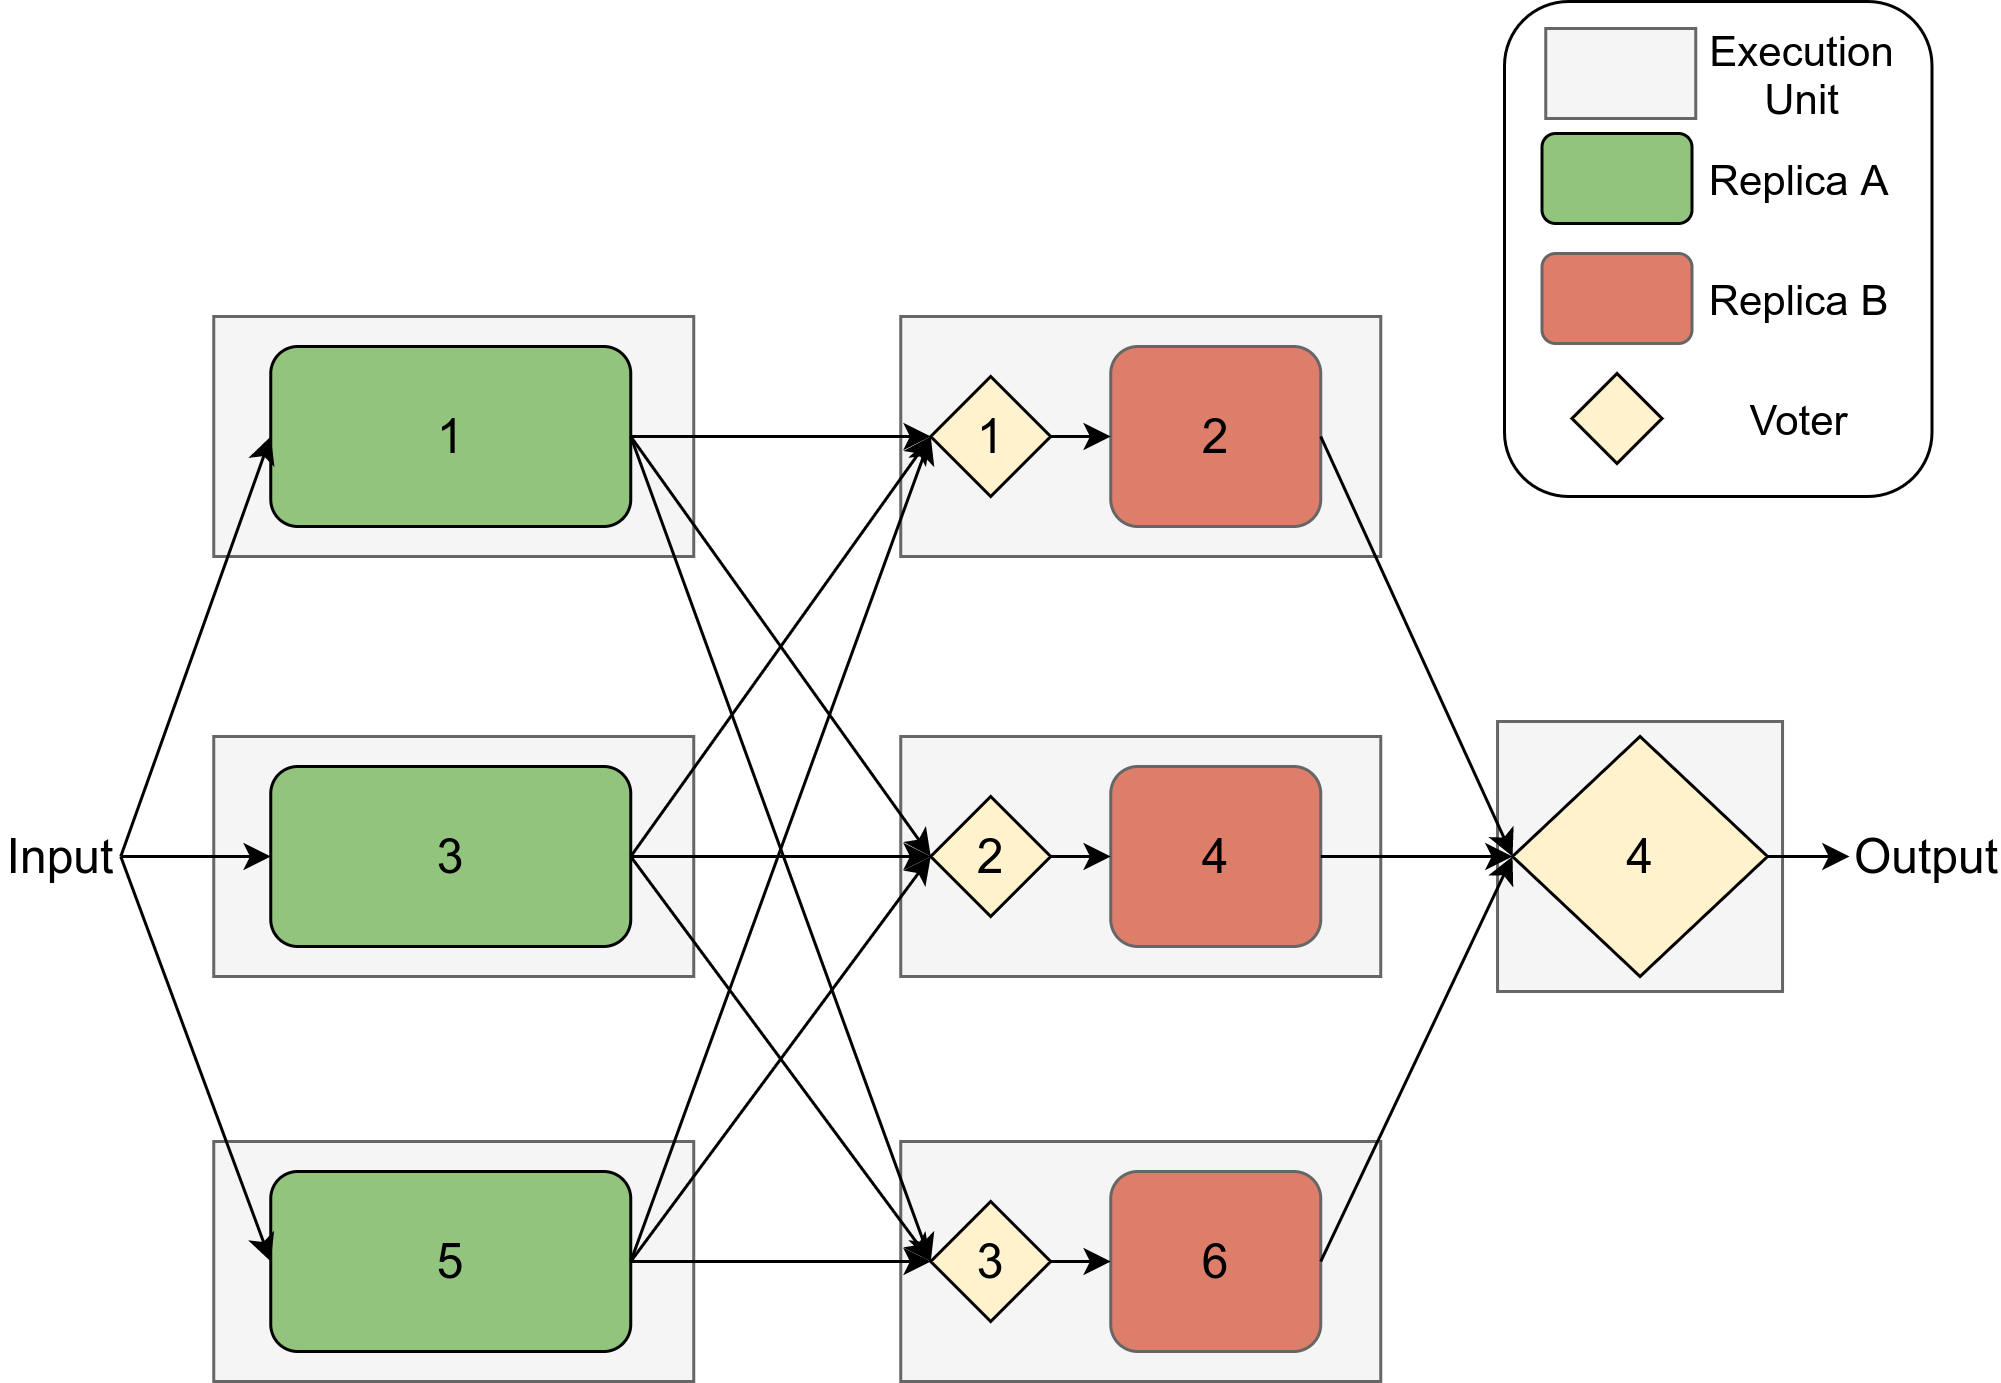
\includegraphics[width=0.75\linewidth]{images/InterconnectedVoterPipeline}
	\caption{Two interconnected pipeline streams with on-component intermediate voting can improve throughput and fault-tolerance.}
	\label{fig:PipelineIntermediateVoters}
\end{figure}

In order to reduce the effect of errors on partial results, an intermediate voting can be applied, as shown in~\autoref{fig:IntermediateVoting}.
Intermediate voting has the additional benefit of introducing pipeline processing into the redundant architecture, so that inputs can be processed step by step.
Thereby, throughput can be enhanced and more inputs can be processed in a given timeframe.
It is also possible that a component functions both as a voter and a data processor, as depicted in~\autoref{fig:PipelineIntermediateVoters}.
This allows voter one, two and three to decide on the intermediate results from replica one, three and five.
The replicas two, four and six can subsequentially work with preselected intermediate result before a final decision is made by voter four.
While the pipelined approach enhances the system's thoughput, it also enhances the computation and communication overhead, as well as the system's cost.
It would also be possible to implement a pipeline-based redundancy approach without intermediat voting.
However, this could lead so situations where a failure in replica (1), (3) and (5) can propagate though the system until a final decision has to be made.

The pipelined system's reliability and fault-tolerance is equal to the non-pipelined one, because at most one replicas of type (A) or (B) are allowed to fail for the system to remain safe.
A tradeoff needs to be made between the added throughput and the additional computation and communication overhead, as well as the increased cost for the system.

So far, all reliability evaluations where made without evaluating the voter, but the voter is the system's weak point because it consitiutes a single point of failure.
As Arifeen \etal showed, the entire system's reliability cannot be higher than the voter's reliability.
One way to solve this would be to dedicate one replica to additionally monitor the voter.
This could be either done by using heartbeat messages, or by demanding a confirmation from the voter.
Thereby, the dedicated replica can detect a possible voter failure and can transition the system into a safe state.
Another way to bypass the voter single-point-of-failure problem is through consensus.

\subsection{Consensus-inspired Architectures}
\begin{figure}[!hb]
	\centering
	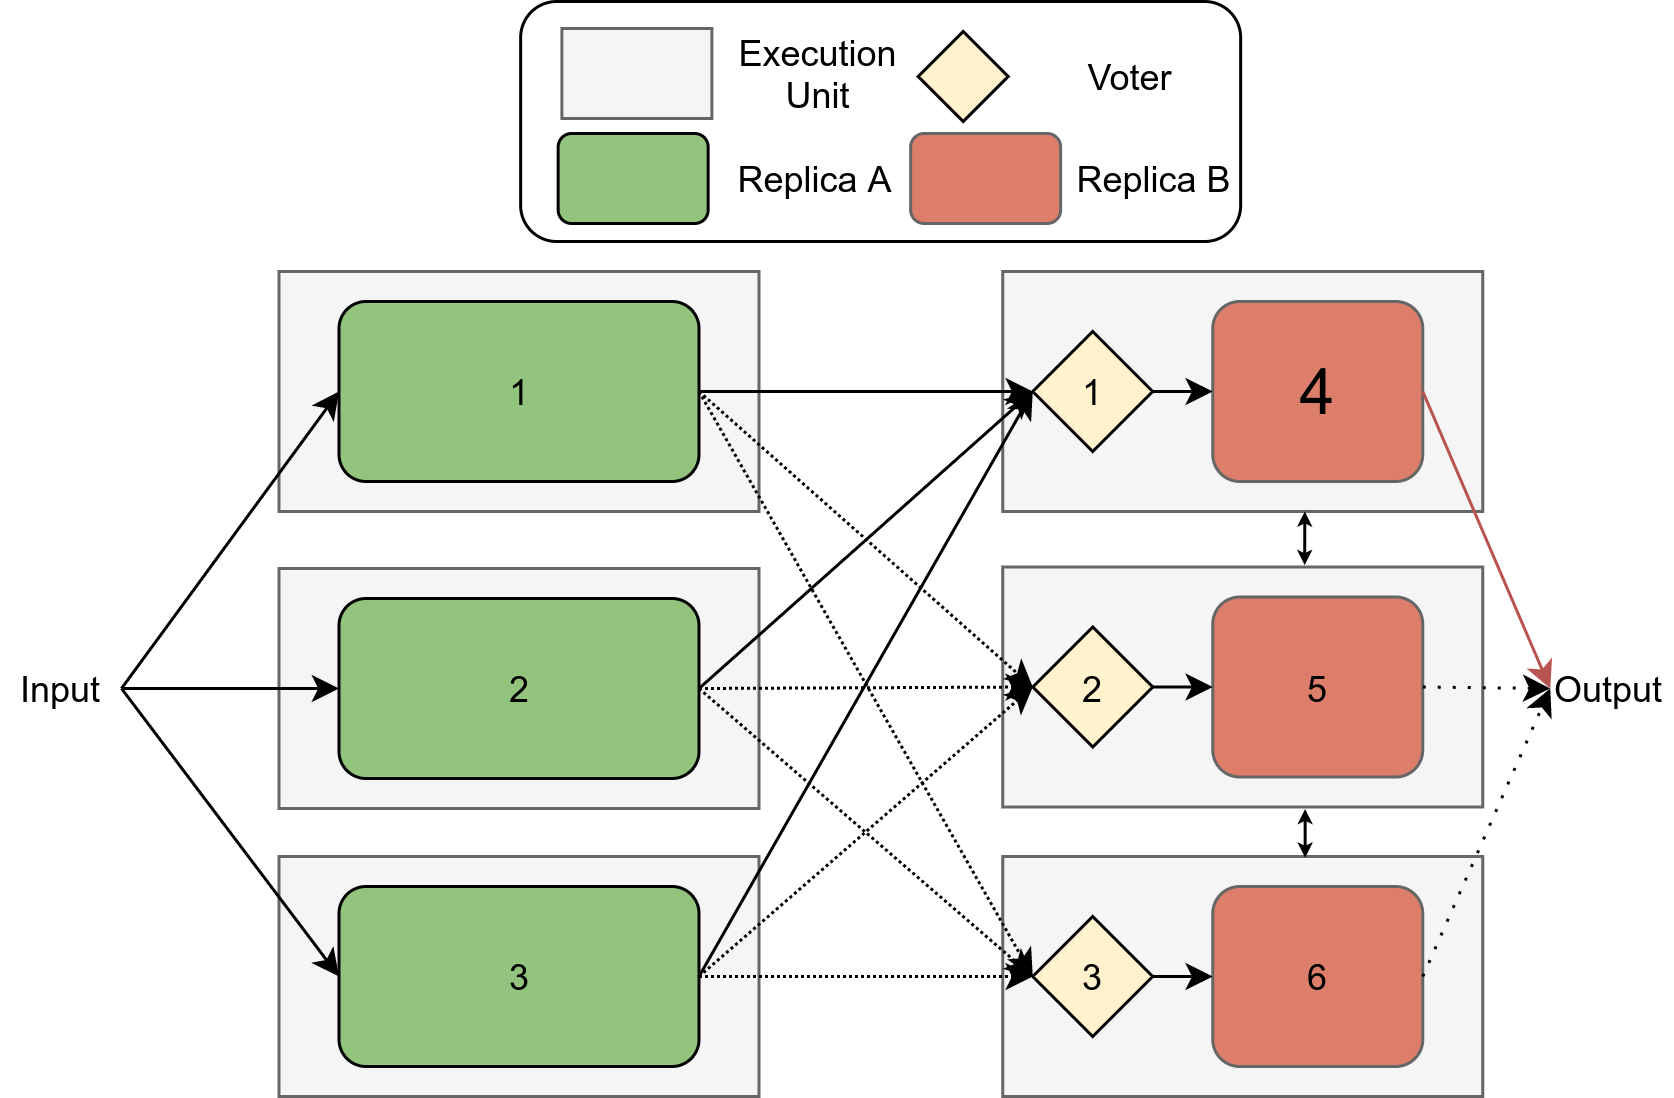
\includegraphics[width=0.75\linewidth]{images/ThreeComponentConsensus}
	\caption{An alternative to a voter can be a consensus algorithm. In this example, which follows basic ideas from \texttt{Raft}, replica (5) with voter (2) took over the leader role.}
	\label{fig:ThreeRepConsensus}
\end{figure}

A spare voter, similar to the spare replica approach described above, cannot be used without any additional concepts.
This is because it required a system wide decision about the fact that the voter crashed.
Either another voter could be used to make this decision, so nothing would be gained by this approach, or a consensus could be made among a subset of components.
For a consensus, multiple components are involved in deciding about redundant information.
An example, where three replicas are involved in finding a consensus, is depicted in~\autoref{fig:ThreeRepConsensus}.
The replicas (1), (2) and (3) build a \abr{TMR}-system, while replicas (4), (5), and (6) are used to find a consensus.
The voters (1), (2) and (3) can collect the redundant results and use majority voting to decide about a value.
A individual replica of type B, together with its voter, takes leadership and decides about the final resulting value.
In the example from~\autoref{fig:ThreeRepConsensus}, replica (5) took over the leader role.
When the component running replica (5) crashes, either the component running replica (4) or replica (6) can take over the voting.
When the new leader also crashes, the last remaining one can transfer the system to a safe state.
\\

An exemplary consensus algorithm that implements the concepts described above, is \texttt{Raft}, which has been proposed by Ongaro and Ousterhout~\cite{RaftConsensusPaper}.
A component in \texttt{Raft} can take on one of three roles, namely \textit{leader}, \textit{follower}, or \textit{candidate}.
There should only be one leader and all other components are followers.
While the leader handles all requests, the followers are passive and only respond to requests from leaders or candidates.
The candidate role is only used when a new leader is about to be elected.
A leader's reachability is verified using heartbeat messages with a specific periodical length, called the \textit{election timeout}.
When the heartbeat message was not received by a follower, it assumes the leader to be down and can react properly.
\\

A fault-tolerant voting approach can be implemented by following \texttt{Raft's} leader concept and two additional \abr{DDS} topics, being two event topics.
One of these topics is used for periodic heartbeat messages and one is used for initiating a new leader election.
The heartbeat topic should use an appropriate deadline and the durability should be set to transient, so that even late joining components know about an existing leader.
The topic for initiating leader election does not require any deadline and the durability can be set to volatile.
\\

The concept described above can be further improved by adding additional \abrpl{RPC}s, as suggested by Raft, in order to instruct the other components and voters to perform voting and reply with the result.
Thereby, a voting on previously voted values can be made by the leader which can eradicate transmission or component failures but increases communication and computation complexity.


%Fischer, Lynch, and Paterson showed, that there exist no consensus algorithm for completely asynchronous systems that can tolerate even a single participant to fail~\cite{FLPProblemConsensus}.
%Thus, a way of synchronizing the system needs to be found to solve the single point of failure problem.
%- Idea: When input is DDS topic, the time at which a new system architecture and a new leader takes over can be done based on the input timestamp
%\todo{Discuss what can be done to improve the voter's reliability}

\subsection{Information and Time}
- How can Information and Time redundancy be used


\section{Final Architecture}


